% Preamble
\documentclass[12pt]{article}

% Packages
\usepackage[left=3.0cm, right=1.5cm, top=2.0cm, bottom=2.0cm]{geometry}

\usepackage[utf8]{inputenc}
\usepackage[T2A]{fontenc}
\usepackage[russian]{babel}
\usepackage{amsmath, amsfonts, amssymb}
\usepackage{graphicx}
\usepackage{wrapfig}
\usepackage{fancyhdr}
\usepackage[shortlabels]{enumitem}
\usepackage{svg}
\usepackage{amstex}
\usepackage{colortbl}
\usepackage{bm}

\renewcommand{\vec}{\textbf}
\newcommand{\cross}{\times}

\pagestyle{fancy}
\fancyhead[L]{Работа №4.4.4}
\fancyhead[R]{Белинский Т.Д.\quad Б05-206}

% Document
\begin{document}
    \section*{4.4.4. ИНТЕРФЕРОМЕТР ФАБРИ-ПЕРО}
    \ \par
    \textbf{Цель работы:} измерение длины волны жёлтых линий ртути, жёлтого дублета натрия,
    определение спектральных характеристик интерферометра Фабри—Перо.

    \textbf{Оборудование:} интерферометр Фабри—Перо, линзы, светофильтры, ртутная и натриевая лампы, катетометр КН-6.

    \subsection*{Теоретическая часть}
    \ \par
    \begin{wrapfigure}{l}{0.4\linewidth}
        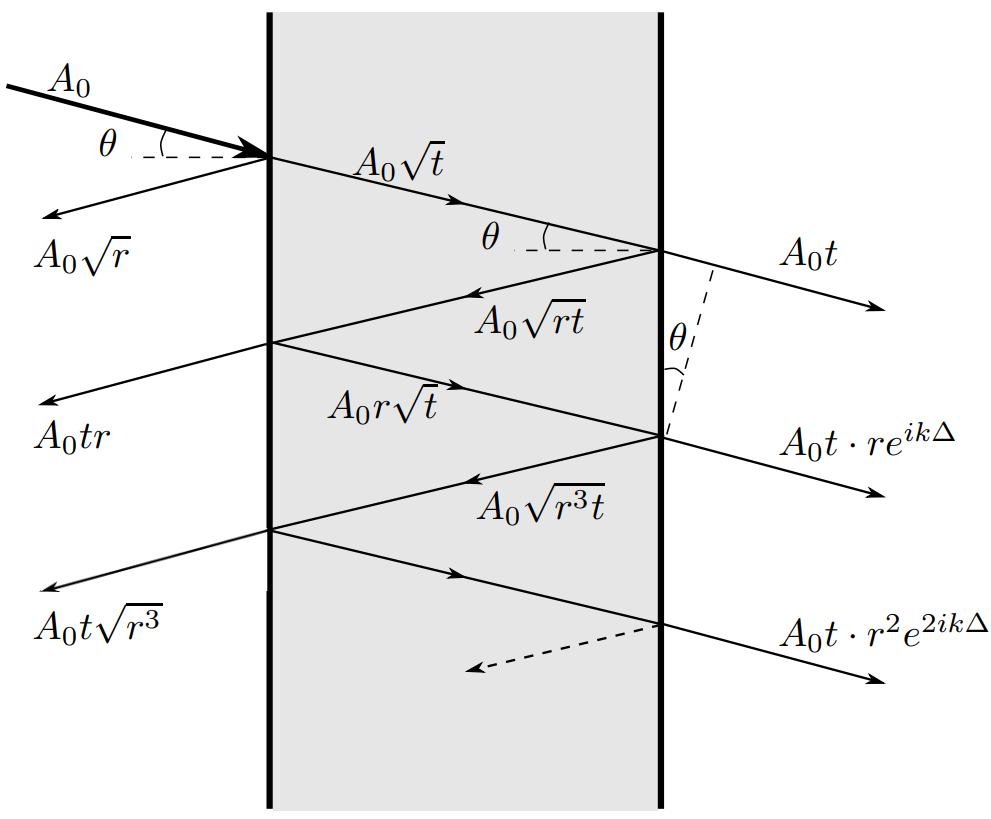
\includegraphics[width=\linewidth]{pic/ifp}
        \caption{Амплитуды волн в интерферометре Фабри-Перо}
        \label{fig:fig1}
    \end{wrapfigure}
    Как спектральный прибор высокой разрешающей способности
    интерферометр Фабри–Перо широко используется в физических экспериментах.
    Он применяется для исследования тонкой структуры спектральных линий,
    является неотъемлемым элементом лазера, выполняя роль оптического резонатора, и т. д.
    Интерферометр Фабри–Перо состоит из двух стеклянных или кварцевых пластин
    с хорошо отполированными поверхностями (с шероховатостью до $10-2\lambda$),
    которые установлены параллельно друг другу на некотором расстоянии.
    На одну поверхность каждой пластины нанесены хорошо отражающие свет покрытия.
    Для получения коэффициента отражения $r \approx 0.9$
    используют металлические покрытия (Ag, Al), для достижения $r \approx 0.99$
    наносятся многослойные диэлектрические интерференционные покрытия.
    Интерферометр Фабри–Перо можно рассматривать как плоскопараллельную пластину,
    в которой происходят многократные отражения и интерференция световых волн.
    На рис.\ \ref{fig:fig1} приведена схема интерферирующих волн.
    Коэффициенты пропускания и отражения по интенсивности отдельного зеркала интерферометра
    равны $t$ и $r$ соответственно (из закона сохранения энергии следует, что $t + r = 1$).
    Пусть $A_0$ -- амплитуда падающей на интерферометр волны,
    тогда амплитуда отражённой от первого зеркала волны равна $A_0\sqrt{r}$,
    амплитуда прошедшей внутрь интерферометра волны -- $A_0\sqrt{t}$,
    амплитуда волны, отражённой от второго зеркала, — $A_0\sqrt{rt}$,
    амплитуда первой прошедшей волны равна $A_0t$ и т. д.
    В результате многократных переотражений на выходе интерферометра будем иметь набор волн,
    амплитуды которых равны $A_0t$, $A_0tr$, $A_0tr^2, \dots$.
    Фазовая задержка между двумя «соседними» волнами равна $k\Delta$, где $k = 2\pi/\lambda$
    -- волновое число; $\Delta$ -- разность хода для угла падения $\theta$.
    Интерференционная картина, наблюдаемая с помощью зрительной трубы, настроенной на бесконечность,
    состоит из концентрических колец равного наклона.
    Найдём условие возникновения интерференционной картины для световой длины волны $\lambda$.
    Выразим разность хода двух интерферирующих волн, падающих на интерферометр под углом $\thtes$:
    \begin{equation}
        \Delta = 2L\left(\frac{1}{\cos\theta} - \tan\theta \sin\theta\right) = 2L\cos\theta,
        \label{eq:eq1}
    \end{equation}
    где $L$ -- расстояние между зеркалами, или \textsc{база интерферометра}.
    Интерференционные максимумы будут наблюдаться для волн, падающих под углами $\theta_m$,
    удовлетворяющими условию:
    \begin{equation}
        2L \cos\theta_m = m \lambda.
        \label{eq:eq2}
    \end{equation}

    Просуммируем комплексные амплитуды световых волн, прошедших интерферометр.
    Можно видеть, что амплитуды прошедших волн образуют геометрическую прогрессию.
    Считая её бесконечной, получим комплексную амплитуду суммарной прошедшей волны:
    \[A = \frac{A_0t}{1 - r \exp^{ik\Delta}}\]
    и ее интенсивность:
    \begin{equation}
        I = |A|^2 = \frac{|A_0|^2t^2}{1 + r^2 - 2r\cos(\frac{4\pi}{\lambda}L\cos\theta)} =
        \frac{I_0}{1 + \frac{4r}{(1 - r)^2} \sin^2(\frac{2\pi}{\lambda}L\cos\theta)}.
        \label{eq:eq3}
    \end{equation}
    Угловое расстояние между парами уменьшается при увеличении угла наблюдения или уменьшении порядка спектра.
    Кроме того, уменьшается расстояние между кольцами в одном порядке и их ширина.

    Угловая дисперсия ИФП оценивается формулой
    \begin{equation}
        D = \frac{d\theta}{d\lambda} = -\frac{m}{2L\sin\theta_m} \approx -\frac{1}{\lambda \theta_m.}
        \label{eq:eq4}
    \end{equation}

    Дифракция Фраунгофера на апертуре интерферометра также влияет на ширину интерференционного кольца
    и разрешающую способность.
    Строго говоря, имеет значение не размер освещённой области зеркала,
    а размер её однородно обработанного участка.
    Напомним, что погрешность обработки и настройки базы интерферометра $L$
    должна быть много меньше $\lambda$.

    Мы ограничимся рассмотрением зависимости разрешающей способности интерферометра Фабри–Перо
    от величины базы $L$ (порядка спектра) и коэффициента отражения зеркал $r$,
    определим угловое расстояние между двумя близкими линиями, соответствующее условию Релея.
    Пусть, как и в случае дифракционной решётки, две линии пересекаются на уровне
    половинной мощности каждой линии.
    Запишем это условие для угла $\theta_m +\delta\theta/2$
    (угол $\theta_m$ соответствует максимуму для длины волны $\lambda$ порядка $m$).
    Используя равенство (\ref{eq:eq3}), имеем
    \[\frac{4r}{(1 - r)^2} \sin^2\left(\frac{\pi}{\lambda}2L\cos(\theta_m + \delta \theta/2)\right) = 1.\]
    Учитывая условие резонанса (\ref{eq:eq2}) и малось углов, получаем
    \[\sin^2\left(\frac{\pi}{\lambda}2L\cos(\theta_m + \delta \theta/2)\right) =
    \sin^2 \left(\frac{2\pi}{\lambda}\cos\theta_m -
    \frac{\pi L}{\lambda}\sin\theta_m \cdot \delta \theta\right) \approx
    \left( \frac{\pi L}{\lambda} \theta_m \delta \theta \right)^2.\]

    Пусть угловому радиусу $\theta_m + \delta\theta$ соответствует максимум интерференционного кольца
    с тем же порядком спектра m и длиной волны $\lambda+\delta\lambda$
    (при пересечении двух линий на уровне половинной мощности угловое расстояние
    между максимумами линий в два раза больше полуширины отдельной линии).
    Величину $\delta \lambda$ можно определить, используя выражение для угловой дисперсии (\ref{eq:eq4}):
    \[\delta \theta = \frac{1- r}{2\pi \sqrt{r}} \frac{\lambda}{2L}\frac{1}{\theta_m}\approx
    D\delta\lambda/2 = \frac{m}{4L\theta_m} \delta\lambda.\]
    Разрешающая способность для порядка спектра $m \approx 2L/\lambda$ равна
    \begin{equation}
        R = \frac{\delta \lambda}{\lambda} \approx \frac{\pi \sqrt{r}}{1 - r}m.
        \label{eq:eq5}
    \end{equation}

    \subsection*{Экспериментальная установка}
    \ \par
    Схема экспериментальной установки приведена на рис.\ \ref{fig:fig2}.
    Свет от лампы $S$, пройдя через линзу $\text{Л}0$ и светофильтр $C$, попадает на интерферометр Фабри—Перо (ИФП).
    Линза $\text{Л}0$ служит для формирования пучка лучей (слегка сходящегося или слегка расходящегося).
    Интерференционные кольца наблюдаются в фокальной плоскости линзы $Л$.
    Картина рассматривается через зрительную трубу $T$, сфокусированную на эту плоскость.
    Диаметры колец измеряются с помощью микроскопа катетометра.
    Зрительная труба $Т$, отсчётный микроскоп — элементы катетометра — прибора,
    предназначенного для измерения расстояний в вертикальной плоскости вдоль вертикальной оси.


    \begin{figure}[h]
        \centering
        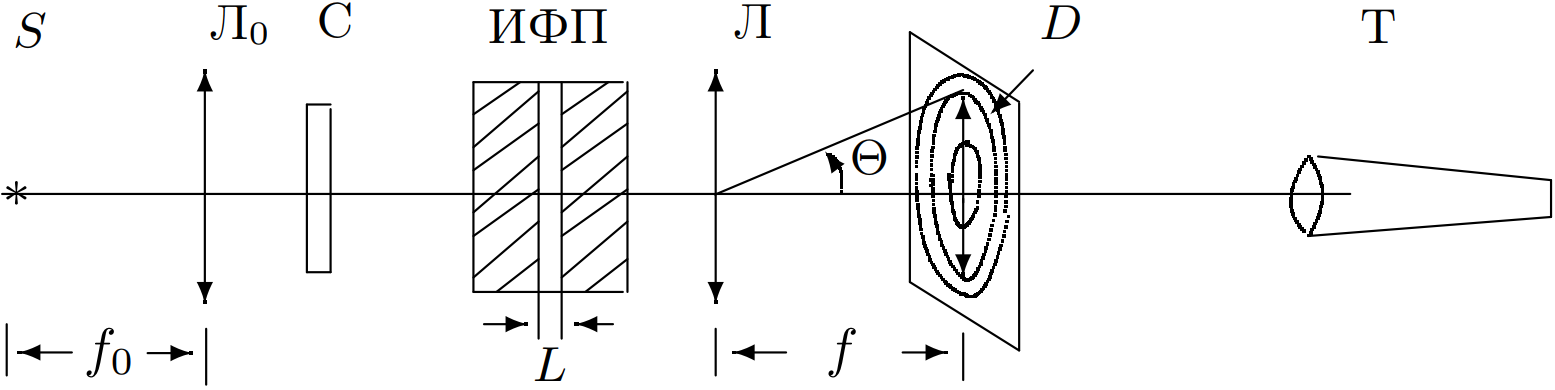
\includegraphics[width=\linewidth]{pic/setup}
        \caption{Схема экспериментальной установки}
        \label{fig:fig2}
    \end{figure}



    \subsection*{Результаты и обработка}
    \begin{enumerate}
        \item
    \end{enumerate}

    \subsection*{Выводы}
    \begin{itemize}
        \item
    \end{itemize}
\end{document}